\documentclass[letterpaper]{article}
\usepackage[spanish]{babel}
\selectlanguage{spanish}
\usepackage[utf8]{inputenc}

\usepackage{lipsum}
\usepackage{amsmath,amssymb,amsfonts,amsbsy}
\usepackage{array}
\usepackage{graphicx}
\usepackage{subfigure}
\usepackage{float}
\usepackage[hidelinks]{hyperref}
\usepackage{ragged2e}

\graphicspath{ {./figures/} }

%\usepackage[pass]{geometry}
\usepackage[left=1.25in,right=1.25in,top=1.0in,bottom=1.0in]{geometry}
\usepackage{listings}

% Custom colors
\usepackage{color}
\definecolor{deepblue}{rgb}{0,0,0.65}
\definecolor{deepred}{rgb}{0.7,0,0}
\definecolor{deepgreen}{rgb}{0,0.6,0}

\usepackage{pgfplots}



\newcommand{\mytitle}{Informe}
\newcommand{\myauthor}{Grupo 24}
\newcommand{\mydate}{\today}


\makeatletter
\renewenvironment{thebibliography}[1]
     {\section{\bibname}% <-- Cambiado de \chapter* a \section*
      \@mkboth{\MakeUppercase\bibname}{\MakeUppercase\bibname}%
      \list{\@biblabel{\@arabic\c@enumiv}}%
           {\settowidth\labelwidth{\@biblabel{#1}}%
            \leftmargin\labelwidth
            \advance\leftmargin\labelsep
            \@openbib@code
            \usecounter{enumiv}%
            \let\p@enumiv\@empty
            \renewcommand\theenumiv{\@arabic\c@enumiv}}%
      \sloppy
      \clubpenalty4000
      \@clubpenalty \clubpenalty
      \widowpenalty4000%
      \sfcode`\.\@m}
     {\def\@noitemerr
       {\@latex@warning{Empty `thebibliography' environment}}%
      \endlist}
\makeatother

\begin{document}
\pagenumbering{gobble}
\begin{minipage}[t]{.13\textwidth}
	\vspace{-0.25in}
	\begin{figure}[H]
		
\includegraphics[width=0.90\textwidth]{imagenes/LogoUC.jpg}
	\end{figure}
\end{minipage}
\hfill
\begin{minipage}[t]{.85\textwidth}
	\vspace{0pt}
	\begin{flushleft}
		\begin{tabular}{l}
			{\sc Pontificia Universidad Cat\'olica de Chile}         \\
			{\sc Escuela de Ingenier\'ia}                            \\
			{\sc Departamento de Ingenier\'ia Industrial y Sistemas} \\
			{\sc ICS1113-Optimizaci\'on}
		\end{tabular}
	\end{flushleft}
\end{minipage}
\vspace{0pt}
\hfill
\vspace*{6cm}
\begin{center}{}
	\vspace*{2mm}
	{\Huge\bf Informe 4}\\
	\vspace*{4mm}
	\hrule\vspace*{1pt}\hrule
	\vspace*{4mm}
	{\LARGE\bf Optimizar la posici\'on de electrolineras y su rentabilidad para Copec en la ciudad de Concepción, Chile}\\
	\vspace*{4mm}
	{\huge\bf Grupo 24 }\\
	\vspace*{1mm}
\end{center}

\vspace*{50mm}
\flushright

Gabriel Cornejo 23647086 Sección 1\\
Sebastián Lorca 23200316 Sección 2\\
Pablo Rojas 23645016 Sección 1\\
Benjamín Sánchez  23205873 Sección 1\\
Víctor Ruiz 2320012J Sección 1\\


\vspace*{5mm}
{\large Fecha entrega: 21 de Junio de 2024\\}

\newpage
\begin{flushleft}
	\tableofcontents
\end{flushleft}

\newpage
\begin{flushleft}
	\listoftables
	\listoffigures
\end{flushleft}

\newpage
\pagenumbering{arabic}
\begin{flushleft}

	\section{Descripción del Problema}
	\subsection{Contexto y beneficios de resolver el problema}
	\justifying
	% Contexto -> Como Copec se enfrenta al desafío de optimizar el posicionamiento de sus centros de carga para vehículos eléctricos (CVE).
	% Mejorar la rentabilidad de estaciones de carga eléctrica para beneficio de la empresa y para masificar la adopción de vehículos eléctricos.
	La transición energética es tema mundial por la importancia de generar un cambio a corto plazo en materia ambiental. En esta línea, Chile tiene metas propuestas para reducir la huella de carbono y para ello, uno de los principales desafíos es en materia automotriz, donde los automóviles eléctricos están cada vez más presentes y se proyecta que para el año 2050 el 40 \% de los vehículos de uso particular sean eléctricos. \cite{Gobierno 1} \\
	Esta proyección se está cumpliendo, ya que se ha visto un crecimiento acorde a lo esperado. Por ejemplo, según datos del sitio Statista en Chile las ventas de autos eléctricos han aumentado considerablemente, teniendo el año 2022, 1295 ventas, que representa más del 200 \% respecto al año 2021 y más del 500\% respecto al 2019. Statista. (2023, 15 octubre). \cite{Gobierno 2} \\


	Entonces, en este contexto de transición hacia una movilidad más sostenible, Copec, una empresa chilena líder en la distribución de combustibles en América Latina, ha decidido incursionar en el mercado de vehículos eléctricos con su plan de movilidad sustentable (Copec Voltex, s.f.) \cite{copec}. Este plan consiste en la implementación de electrolineras, que son puntos de carga públicos para BEV1 a lo largo de todo Chile, para hacer posible una red conectada, donde usuarios puedan desplazarse sin depender de la autonomía de su EV2.
	Uno de los mayores desafíos presentes en esta iniciativa es lograr optimizar el posicionamiento de sus centros de carga para vehículos eléctricos (CVE). Este proceso implica identificar las ubicaciones óptimas para instalar estos centros de carga, considerando diversos factores como la demanda potencial, la infraestructura eléctrica disponible, la accesibilidad y la rentabilidad económica. \\

	El tomador de decisiones en este caso es el equipo de planificación estratégica de Copec Voltex, que busca maximizar la rentabilidad de los centros de carga eléctricos en Chile, satisfaciendo la creciente demanda de vehículos eléctricos. El horizonte de planificación adecuado abarca al menos un período de 5 años, ya que se espera que la adopción de vehículos eléctricos continúe en aumento durante este tiempo.

	Resolver este desafío le entregará a Copec Voltex la iniciativa de aumentar la cantidad de electrolineras, lo que, a su vez, no solo facilitará el acceso a esta tecnología emergente, sino que puede impulsar la adopción de esta tecnología al reducir las barreras de acceso para los conductores. De esta manera, lo que contribuirá significativamente a la reducción de emisiones contaminantes y al combate del cambio climático que es justamente el compromiso de Copec con su comunidad. \\

	Actualmente, Copec Voltex cuenta con una red de carga de 68 electrolineras en la Región Metropolitana, y 128 puntos a lo largo de todo el país. Eso significa una conexión de 1400 kilómetros, según indican en su sitio (Copec Voltex, s.f.). Sin embargo, tras un análisis de la autonomía de los EVs en promedio, y las distancias entre electrolineras en Chile, algunos EVs económicos como el Mazda MX-30 EV no logran cruzar las distancias entre electrolineras (Scheer, 2022) \cite{scheer}. Por esto, un modelo que sea capaz de encontrar una solución de red para todo vehículo se hace necesaria. \\

	Continuando en este eje, según una encuesta realizada por el diario la Tercera el 15\% de los encuestados cree que una de las barreras para adquirir un vehiculo electrico es la que la red de carga no avanza del todo de acuerdo a lo esperado \cite{Tercera}. Respecto a este desafío ya conocido Diego Pardow, el ministro de energía habló sobre la Hoja de Ruta para el Avance de la Electromovilidad en Chile, donde uno de los ejes estratégicos para incentivar el uso de vehículos eléctricos es precisamente mejorar la red de carga.

	Es en esta línea que se considera de gran valor el problema a optimizar, ya que, según Diego Mendoza, secretario general de ANAC (Asociación Nacional Automotriz de Chile) el parque electrificado a la fecha de septiembre del 2023 es de 4610 vehículos, y se espera que para el año 2025 el 5\% del mercado Automotriz sea de vehículos eléctricos. Tomando datos anteriores, en el año 2023 se comercializaron 313.865 vehículos \cite{chileautos} mientras que en el año 2022 la cifra fue de 426.772 \cite{Tercera-1}. Suponiendo que en el año 2025 en el mercado habran 350.000 vehículos en el mercado, si se cumple la proyección esperada se estarían comercializando 17.500 vehículos eléctricos aproximadamente. A su vez, asumiendo que habr\'a un crecimiento lineal de comercializaci\'on de veh\'iculos el\'ectricos y considerando los que ya hay en circulaci\'on, se puede estimar que para el año 2025 habr\'ian alrededor de 30.000 vehículos eléctricos en circulación lo cual representa el 650\% de la cantidad actual. Siguiendo en esta línea, considerando que Copec tiene la mayor implicancia en el mercado de puntos de carga para EVs para el año 2025, se habr\'ia ayudado a más de 10.000 vehículos eléctricos generando una red de puntos de carga óptima acorde al crecimiento esperado y que se está desarrollando en el país.
	\subsection{Objetivo que persigue el tomador de decisiones}
	El equipo de planificación de Copec Voltex busca maximizar la rentabilidad y promover la electromovilidad. Para lograr este objetivo, el tomador de decisiones evaluará diversos aspectos, incluida la cantidad óptima de cargadores a comprar por período considerando el costo y la demanda. También determinará el momento y lugar adecuados para instalar infraestructura de carga, teniendo en cuenta los requisitos específicos de cada ubicación y las restricciones, como la distancia entre estaciones para respetar la autonomía de los vehículos eléctricos. Además, se administrará el inventario de manera eficiente para garantizar un suministro adecuado. Todas estas decisiones se tomarán considerando los costos asociados y las restricciones necesarias para garantizar una solución realista y óptima

	\section{Modelación del problema}
	\subsection*{Supuestos}
	\begin{itemize}
		\item La cantidad de estaciones existente no supera la capacidad máxima de la infraestructura eléctrica.
		\item Los \textit{EV}s van a cargar en promedio $\delta$ KW en un mes.
		\item La demanda total se considerar\'a como la cantidad de veh\'iculos disponibles en la regi\'on.
	\end{itemize}
	\subsection{Conjuntos}
	\begin{itemize}
		\item $t \in \{1, \ldots, 60\}$, el mes desde la implementación del modelo.
		\item $i \in I$, donde $I$ es el conjunto de ubicaciones de los posibles centros de carga.
		\item $m \in M$, donde $M$ es el conjunto de tipos de cargadores.
	\end{itemize}

	\subsection{Parámetros}
	\begin{itemize}
		\item $D_{mit}$, demanda total de cargadores tipo $m$ en la estación $i$ para el periodo $t$.
		\item $CI_{it}$, el costo de instalar la infraestructura el\'ectrica en el periodo $t$ para la estaci\'on $I$.
		\item $CP_{mt}$, el costo de comprar un cargador tipo $m$ en el periodo $t$.
		\item $CC_{mit}$, el costo de instalar un cargador tipo $m$ en la estación $i$ en el periodo $t$.
		\item $CKW_{mit}$, el costo de energía eléctrica por kilowatt-hora para un cargador tipo $m$ en la estación $i$ en el periodo $t$.
		\item $CM_{mit}$, el costo de mantención de un cargador tipo $m$ en la estación $i$ en el periodo $t$.
		\item $\alpha$, coeficiente de ganancia espera por el precio seleccionado, por KW de electricidad vendido.
		\item $\delta$, cantidad de KW que se espera que cargue un vehículo eléctrico en un mes.
		\item $\phi_m$, capacidad de carga por mes de un cargador tipo $m$ en KW.
		\item $K$, la capacidad eléctrica máxima que permite la infraestructura eléctrica.
		\item $EI_{i}$, si ya existe la infraestructura eléctrica en la estación $i$.
		\item $EC_{mi}$, la cantidad de estaciones de carga de tipo $m$ que ya existen en la estación $i$ en el mes $t$
		\item $CS_{mt}$, el costo de almacenar un cargador tipo $m$ en el periodo $t$.
		\item $AM$, la distancia máxima permitida entre electrolineras.
	\end{itemize}
	\subsection{Variables de decisión}
	\begin{itemize}
		\item $x_{mit}$ cantidad de cargadores tipo $m$ en la estación $i$ para el periodo $t$.
		\item \[
			      y_{it} =
			      \begin{cases}
				      1 & \quad\text{si se instala la infraestructura eléctrica para }i\text{ en }t \\
				      0 & \quad\text{en cualquier otro caso.}
			      \end{cases}
		      \]
		\item \[
			      z_{it} =
			      \begin{cases}
				      1 & \quad\text{si existe la infraestructura eléctrica para }i\text{ en }t \\
				      0 & \quad\text{en cualquier otro caso.}
			      \end{cases}
		      \]
		\item $a_{mt}$, cantidad de cargadores tipo $m$ que se compran en el periodo $t$.
		\item $b_{mit}$, cantidad de cargadores tipo $m$ que se instalan en la estación $i$ en el periodo $t$.
		\item $d_{mit}$, (Cant. de vehiculos)demanda que se va a satisfacer para cargadores tipo $m$ en la estación $i$ en el periodo $t$.
		\item $S_{mt}$, cantidad de cargadores almacenados de tipo $m$ el periodo $t$.
	\end{itemize}
	\subsection{Función Objetivo}
	\begin{center}
		$\max \; \sum_{m \in M}\sum_{i \in I} \sum_{t=1}^{60} (d_{mit} \cdot CKW_{mit} \cdot (\alpha - 1) - x_{mit} \cdot CM_{mit} - b_{mit} \cdot CC_{mit}) - \sum_{t \in T} \sum_{m \in M} a_{mt} \cdot CP_{mt} - \sum_{t \in T}\sum_{m \in M} CS_{mt} \cdot S_{mt} - \sum_{t \in T} \sum_{i \in I} y_{it} \cdot CI_{it}$
	\end{center}

	\subsection{Restricciones}

	\begin{enumerate}
		\item Restricción de inventario, incluyendo la condici\'on inicial (\textit{storage}).
		      \begin{align*}
			       & S_{m(t-1)} + a_{mt} = S_{mt} + \sum_{i \in I} b_{mit} &  & \forall \; m \in M, t \in \{2, \ldots, 60\} \\
			       & a_{m1} = S_{m1} + \sum_{i \in I} b_{mi1}              &  & \forall \; m \in M
		      \end{align*}
		\item Restricción de cantidad de cargadores instalados ($x$) que solo puede ser mayor a $0$ cuando se instala la infraestructura eléctrica ($y$).
		      \begin{align*}
			       & N \cdot \sum_{t'=1}^{t} y_{it'} \geq x_{mit} &  & \forall \; m \in M, \; i \in I,\; t \in \{1, \ldots, 60\}
		      \end{align*}
		\item S\'olo se puede instalar la infraestructura el\'ectrica una vez si no se ha instalado antes ($EI$).
		      \begin{align*}
			       & \sum_{t \in T} y_{it} \leq 1 - EI_i &  & \forall \; i \in I
		      \end{align*}
		\item La capacidad en KW de los cargadores instalados ($x$) no puede superar la capacidad m\'axima de KW de la infraestructura el\'ectrica ($K$).
		      \begin{align*}
			       & K \geq \sum_{m \in M} x_{mit} \cdot \phi_m &  & \forall \; i \in I, \; t \in \{1, \ldots, 60\}
		      \end{align*}
		\item Solo puede haber infraestructura el\'ectrica en una ubicaci\'on ($z$) si se ha instalado anteriormente ($y$)
		      \begin{align*}
			       & z_{it} \leq \sum_{t'=1}^{t} y_{it'} + EI_i &  & \forall \; i \in I, \; t \in \{1, \ldots, 60\} \\
			       & z_{it} \geq y_{it} + z_{i(t-1)}            &  & \forall \; i \in I, \;t \in \{2, \ldots, 60\}  \\
			       & z_{i1} \geq y_{i1} + EI_i                  &  & \forall \; i \in I
		      \end{align*}
		\item Solo puede haber un centro de carga en una ubicaci\'on $j$ si existe al menos una estaci\'on cuya distancia es menor a la distancia m\'axima permitida ($AM$).
		      \begin{align*}
			       & \sum_{i \in I: i \neq j, d_{ij}\leq AM} z_{it} \geq z_{jt} &  & \forall \; j \in I, \; t \in \{1, \ldots, 60\}
		      \end{align*}
		\item La cantidad de cargadores en una estaci\'on ($x$) debe ser consistente, es decir, debe ser igual a la cantidad instalada en el periodo más la existente en el periodo anterior, considerando la condici\'on inicial.
		      \begin{align*}
			       & x_{mit} = b_{mit} + x_{mi(t-1)} &  & \forall \; m \in M, \; i \in I, \; t \in \{2, \ldots, 60\} \\
			       & x_{mi1} = b_{mi1} + EC_{mi}     &  & \forall \; m \in M, \; i \in I
		      \end{align*}
		\item La demanda a satisfacer, entendida como cantidad de vehículos, no puede superar la demanda total de para el cargador tipo $m$ en la estación $i$ para el periodo $t$.
		      \begin{align*}
			       & d_{mit} \leq D_{mit} &  & \forall \; m \in M, \; i \in I, \; t \in \{1, \ldots, 60\}
		      \end{align*}
		\item La cantidad de KW que se van a proveer para cargadores de tipo $m$ no puede superar la capacidad de carga de los cargadores instalados en la estación $i$ en el periodo $t$.
		      \begin{align*}
			       & \delta \cdot d_{mit} \leq x_{mit} \cdot \phi_m &  & \forall \; m \in M, \; i \in I, \; t \in \{1, \ldots, 60\}
		      \end{align*}
		\item Naturaleza de las variables.
		      \begin{align*}
			       & y_{it}, z_{it} \in \{0, 1\}                             &  & \forall \; i \in I, \; t \in \{1, \ldots, 60\} \\
			       & x_{mit}, a_{mit}, b_{mit}, d_{mit} \in \mathbb{Z}^{+}_0 &  & \forall \; m\in M, i\in I, t\in T
		      \end{align*}
	\end{enumerate}

	\subsection{Naturaleza de las variables}
	\begin{itemize}
		\item $x_{mit}$: Cantidad de cargadores tipo $m$ en la estación $i$ para el periodo $t$. Es una variable entera no negativa.
		\item $a_{mit}$: Cantidad de cargadores tipo $m$ que se compran en el periodo $t$. Es una variable entera no negativa.
		\item $b_{mit}$: Cantidad de cargadores tipo $m$ que se instalan en la estación $i$ en el periodo $t$. Es una variable entera no negativa.
		\item $d_{mit}$: Demanda que se va a satisfacer para cargadores tipo $m$ en la estación $i$ en el periodo $t$. Es una variable entera no negativa.
		\item $y_{it}$: Variable binaria que indica si se instala la infraestructura eléctrica para la ubicación $i$ en el periodo $t$. Toma el valor 1 si se instala la infraestructura y 0 en cualquier otro caso.
		\item $z_{it}$: Variable binaria que indica si existe la infraestructura eléctrica para la ubicación $i$ en el periodo $t$. Toma el valor 1 si la infraestructura existe y 0 en cualquier otro caso.
	\end{itemize}
	\section{Definición de datos}

	Para la recolección y realización de este modelo, se restringe la zona de estudio a la ciudad de Concepción, Chile. Se considera que la ciudad de Concepción es una ciudad de tamaño mediano, con una población de aproximadamente 220.000 habitantes, y una densidad de población de 5.100 habitantes por kilómetro cuadrado \cite {INE}. Además, se considera que la ciudad de Concepción tiene una infraestructura eléctrica adecuada para soportar la instalación de electrolineras, y que la ciudad cuenta con una red de carreteras que conecta los principales puntos de la ciudad.

	\subsection{Demanda de cargadores}

	Considerando que el 53\% de los cargadores électricos se encuentran en regiones \cite{cargadores}, se estimará como un 11\% de este valor para Concepción. Ahora multiplicando 0.11 por el total de vehiculos eléctricos en Chile (900) \cite{autostot}, nos da un total de $\approx 100$ autos en Concepción.

	Así, como se está llevando a cabo una extrapolación de los datos y se debe asumir un margen de error, se tendrá que la cantidad de vehículos variará entre 90 y 110 por período, aumentando exponencialmente en un 1.35\% anual (\cite{incremento-autos}).

	\subsection{Costos}

	\textbf{Costo de Instalación de Infraestructura Eléctrica:} Se estima que el costo de instalar la infraestructura eléctrica en una estación de carga es de \$1.707.077 CLP a \$40.813.109 CLP \cite{infraestructura}. Este rango se debe a que no se pudo recolectar información específica para Copec en Concepción, por lo que tomaremos un rango amplio para contemplar la variabilidad de los costos.

	\textbf{Costo de Compra:} El costo de compra de cada cargador es de \$1.600.000 CLP (IVA incluido), según precio de mercado (\cite{charge-cost}).

	% https://www.electromov.cl/2022/01/12/costo-promedio-para-instalar-infraestructura-de-carga-en-chile-llega-a-los-77-millones/
	% https://xolary.com/potencia-necesaria-para-cargar-tu-coche-electrico/
	%Costo instalación m: 1.800.000 - 5.500.000 $CLP (1 solo cargador) Considerando que un cargador tiene una potencia de 4 a 22 kW
	\textbf{Costo de Instalación de Cargador:} El costo de instalar un cargador de cualquier tipo se mueve en un rango de \$1.800.000 a \$5.500.000 CLP \cite{infraestructura}. Este rango se debe a que no se pudo recolectar información específica para Copec en Concepción, por lo que tomaremos un rango amplio para contemplar la variabilidad de los costos.

	%Costo Kwh/hora: 100 - 200 $CLP
	%Referencias: 
	%https://www.globalpetrolprices.com/Chile/electricity_prices/
	\textbf{Costo de Energía Eléctrica:} El costo de energía eléctrica por kilowatt-hora es de \$100 a \$200 CLP \cite{kwh}. Con esto, se logra un precio competitivo con respecto a los combustibles fósiles y con la opción de implementar un sistema de carga particular.

	%Costo de mantención m: 70.000 - 120.000 CLP (al mes)
	%Referencias: 
	%https://mobilityportal.lat/cuesta-mantener-punto-de-carga/
	\textbf{Costo de Mantención:} El costo de mantención de un cargador es de \$70.000 a \$120.000 CLP al mes \cite{mantencion}.

	\textbf{Costo de Almacenaje:} Se va a considerar, a falta de información precisa, que el costo de almacenar un cargador significará un 10\% a 30\% del costo de compra del mismo. Así, se estima que el costo de almacenar un cargador es de \$50.000 a \$150.000 CLP.
	\subsection{Transformadores}

	\subsubsection{Coeficiente de Ganancia}

	El coeficiente de ganancia es el multiplicador $\alpha$ que se aplica al precio de la electricidad vendida. Así, el precio es calculado en base al costo (haciéndolo lineal) y se le agrega un porcentaje de ganancia. Se estima que el coeficiente de ganancia es de 1.9, ya que COPEC Voltex tiene sus precios en \$295 CLP por KW \cite{copec}.

	\subsubsection{Carga Promedio de KW en un Mes}

	% Cantidad de KW que se espera que cargue un vehículo eléctrico en un mes: 225 - 375 kWh
	%Referencias:
	%https://motor.elpais.com/coches-electricos/cuanto-consume-un-coche-electrico-y-como-calcularlo/
	%https://www.latercera.com/mtonline/noticia/cuanto-cuesta-recargar-un-auto-electrico-es-mas-barato-hacerlo-en-casa-o-en-una-electrolinera/VFLHTHA4YVFHZKRNBX3VL5GNAQ/
	%https://movilidadconelectricidad.com/blog/cuantos-kwh-consume-un-coche-electrico/

	Se estima que la cantidad de KW que se espera que cargue un vehículo eléctrico en un mes es de 225 a 375 kWh en promedio (\cite{delta1} \cite{delta2} \cite{delta3}).

	\subsubsection{Capacidad de Carga por Mes por Cargador}

	Considerando que los cargadores a considerar tienen una potencia de 7 a 22 KW \cite{cargadores}, se estima que la capacidad de carga por mes de un cargador es:

	\begin{align*}
		\phi_m =
		\begin{cases}
			7 [\text{kW}] \cdot 12\; [\text{horas}] \cdot  30 \;[\text{días}] = 2520 \; \text{kWh} & \quad\text{si el cargador es de 7 KW}  \\
			22 [\text{kW}] \cdot 12\; [\text{horas}] \cdot  30 \;[\text{días}] = 7920 \;\text{kWh} & \quad\text{si el cargador es de 22 KW}
		\end{cases}
	\end{align*}

	\subsubsection{Capacidad Estructural Eléctrica Máxima}

	Para las electrolineras se construye una red eléctrica especial, es por esto que su capacidad eléctrica es mucho mayor a la de los particulares y planificada considerando el uso que se le va a dar (junto a su demanda). Por eso, se considera que el máximo de KW por mes que permite la infraestructura eléctrica es de:

	\begin{align*}
		K = \frac{2520 + 7920}{2} \cdot 5= 22.200 \; \text{kWh}
	\end{align*}

	\subsection{Elementos Existentes}

	\subsubsection{Infraestructura Eléctrica}

	Según lo investigado, la infraestructura eléctrica existe para las estaciones 5 y 10, por lo que $EI_i = 0$ para todo $i \in I: i \not \in \{5,10\}$ y $EI_5,EI_{10}=1$.

	\subsubsection{Cargadores Existentes}

	Según lo investigado, existen cargadores en las estaciones 5 y 10, por lo que $EC_{mi} = 0$ para todo $m \in M$ y $i \in I: i \not \in \{5,10\}$. Para la estación 5, $EC_{m5} = 2$ y para la estación 10, $EC_{m10} = 1$.

	\section{Implementación Computacional}

	Para implementar el modelo se requiere contal con el archivo \texttt{parametros.zip} que contiene los datos necesarios para la ejecución del modelo, así como también se requiere \texttt{main.py}. A continuación se detalla el contenido de los archivos:

	\textbf{main.py:} Archivo principal que contiene la implementación del modelo matemático, la lectura de los datos y la ejecución del modelo. Entrega la ganancia esperada al término del horizonte de tiempo.

	\textbf{parametros.zip:} Archivo comprimido que contiene los datos necesarios para la ejecución del modelo. Contiene los siguientes archivos:

	\begin{itemize}
		\item \texttt{demanda/ :} Directorio\footnote{carpeta} que contiene la demanda de cargadores para cada estación en cada mes (cada archivo representa un mes).
		\item \texttt{costo\_inst/ :} Directorio que contiene los costos de instalación de infraestructura eléctrica.
		\item \texttt{costo\_kw/ :} Directorio que contiene costos de la electricidad en CLP.
		\item \texttt{costo\_man/ :} Directorio que contiene los costos de mantención de los cargadores.
		\item \texttt{alpha.csv:} Archivo que contiene el coeficiente de ganancia esperado por el precio seleccionado.
		\item \texttt{AM.csv:} Archivo que contiene la distancia máxima permitida entre electrolineras.
		\item \texttt{capacidad\_carga.csv:} Archivo que contiene la capacidad de carga por mes de un cargador.
		\item \texttt{cargadores\_existentes.csv:} Archivo que contiene la cantidad de cargadores existentes en cada estación.
		\item \texttt{costo\_almacenamiento.csv:} Archivo que contiene el costo de almacenar un cargador en cada período.
		\item \texttt{costo\_compra.csv:} Archivo que contiene el costo de compra de un cargador en cada período.
		\item \texttt{costo\_instalacion\_electrica.csv:} Archivo que contiene el costo de instalar la infraestructura eléctrica en cada período.
		\item \texttt{delta.csv:} Archivo que contiene la cantidad de KW que se espera que cargue un vehículo eléctrico en un mes.
		\item \texttt{distance.csv:} Archivo que contiene la distancia real entre electrolineras.
		\item \texttt{infraestructura\_existente.csv:} Archivo que contiene si ya existe la infraestructura eléctrica en la estación.
		\item \texttt{K.csv:} Archivo que contiene la capacidad eléctrica máxima que permite la infraestructura eléctrica.
	\end{itemize}

	\textbf{Instrucciones de uso:} Para ejecutar el modelo, se debe descomprimir el archivo \texttt{parametros.zip} y ejecutar el archivo \texttt{main.py} en la misma carpeta que los archivos descomprimidos. El modelo entregará la ganancia esperada al término del horizonte de tiempo.

	\section{Resultados}

	Los gráficos de cada variable se encuentran en \textit{resultados.xlsx}, en la hoja de cálculo de resultados. A continuación, se presentan los resultados obtenidos para cada variable de decisión.

	\subsection{$x_{mit}$}

	Los siguientes gráficos muestran cómo para las 13 estaciones los valores de la variable “x” fueron variando en el tiempo para cada cargador. En el caso del cargador de tipo 1 se puede evidenciar que la evolución de la cantidad de cargadores por estación fue creciente o constante, lo cual es de sumo interés ya que cumple la restricción de que no pueden desaparecer cargadores en el tiempo (restricción 7). Los gráficos están en la hoja \textit{xmit} y los nombres para los gráficos son: \textit{Valores de x para cargador tipo 1} y \textit{Valores de x para cargador tipo 2}.

	\subsection{$y_{it}$}

	En el gráfico es difícil de ver, pero muestra los valores de la variable “y” para cada período de tiempo y para cada estación. Se sabe que se parte con 2 estaciones de 12 habilitadas y que se habilitaron todas las estaciones al final del tiempo, por lo que tiene sentido que la variable solo en un periodo $t$ para cada estación tome el valor 1, ya que solo se puede instalar una vez. Los gráficos están en la hoja \textit{yit} y los nombres para los gráficos son: \textit{Estación 1} y \textit{Estación 2}.

	\subsection{$z_{it}$}

	El gráfico es un poco complejo de leer, pero lo que representa es que la infraestructura una vez que fue instalada, preserva su existencia hasta el final de los periodos, ya que la variable toma el valor 1 en un $t$ y luego se mantiene constante para todas las estaciones. Para facilitar la lectura de la variable \textit{zit}, se presenta el siguiente recurso dinámico: \url{https://stupendous-genie-3fd288.netlify.app/} en el cual se puede observar la instalación de infraestructura por periodo. Los gráficos están en la hoja \textit{zit} y los nombres para los gráficos son: \textit{Infraestructura presente por estación en el tiempo}.

	\subsection{$a_{mt}$}

	En el gráfico se puede observar que hubo compras de cargadores en distintos periodos $t$. Esto, además de demostrar que hubo un gasto en cargadores, se relaciona con las variables \textit{xmit}, que debería aumentar en alguna estación en un periodo donde haya compra ya que no hay almacenamiento, y con la variable \textit{bmit}, que debería también cuando se compran cargadores en un periodo $t$. Los gráficos están en la hoja \textit{amt} y los nombres para los gráficos son: \textit{Cantidad de cargadores comprados en cada periodo}.

	\subsection{$b_{mit}$}

	En este gráfico se muestra la cantidad de cargadores de ambos tipos que se instalan para cada estación en los periodos $t$. Como se mencionó anteriormente, tiene relación directa con \textit{amt}, ya que si se compra en un periodo $t$, en ese mismo periodo debe instalarse en alguna estación $i$ un cargador de ese tipo. Los gráficos están en la hoja \textit{bmit} y los nombres para los gráficos son: \textit{Cantidad de Cargadores Tipo 1 Que Se Instalaron por Estación} y \textit{Cantidad de Cargadores Tipo 2 Que Se Instalaron por Estación}.

	\subsection{$d_{mit}$}

	En el gráfico de esta variable para cada periodo $t$ se puede evidenciar claramente cómo con el tiempo se pudo ir satisfaciendo cada vez más demanda. Esto tiene sentido, ya que a largo plazo había que recuperar los costos que significaron todas las compras e instalaciones en un principio y así poder generar una rentabilidad óptima. Los gráficos están en la hoja \textit{dmit} y los nombres para los gráficos son: \textit{Demanda a satisfacer cargador 1} y \textit{Demanda a satisfacer cargador 2}.

	\subsection{$S_{mt}$}

	Como fue mencionado anteriormente en \S 5.4, no hubo almacenamiento de cargadores ya que el costo de almacenamiento era superior al incremento por periodo del costo de compra. En el siguiente gráfico podemos ver el comportamiento de la satisfacción de demanda para cada periodo $t$ en una estación $i$ para los 2 tipos de cargadores. En el siguiente gráfico podemos ver que la cantidad de cargadores almacenados de ambos tipos en cada periodo tiene una correcta relación con las cantidades que había en los periodos previos y posteriores, cumpliendo nuestra restricción. Los gráficos están en la hoja \textit{Smt} y los nombres para los gráficos son: \textit{Cantidad de Cargadores Almacenados por Periodo}.

	\newpage
	\section{Análisis de Sensibilidad}


	\subsection*{Coeficiente de Ganancia Esperada por el Precio Seleccionado ($\alpha$)}

	\begin{table}[H]
		\centering
		\begin{tabular}{|c|c|c|}
			\hline
			\textbf{Coeficiente de ganancia esperada} & \textbf{Cambio porcentual} & \textbf{Rentabilidad [CLP]} \\
			\hline
			$1.9 \times 70\% = 1.615$                 & -78.37\%                   & \$435,338,090               \\
			$1.9 \times 85\% = 1.615$                 & -40.59\%                   & \$1,195,887,520             \\
			\textbf{Valor original: 1.9}              & \textbf{0\%}               & \textbf{\$2,013,071,275}    \\
			$1.9 \times 115\% = 1.615$                & +41\%                      & \$2,838,576,671             \\
			$1.9 \times 130\% = 1.615$                & +82\%                      & \$3,666,357,631             \\
			\hline
		\end{tabular}
		\caption{Análisis de Sensibilidad del Coeficiente de Ganancia Esperada}
	\end{table}

	Como se puede evidenciar en la tabla anterior, la rentabilidad del modelo es casi completamente lineal con relación al coeficiente de ganancia esperada. Esto era predecible y ahora se confirma como adecuado, ya que cualquier aumento en el coeficiente $\alpha$ resulta en un incremento en las ganancias, afectando positivamente la rentabilidad.

	Además, es crucial notar que el modelo muestra una alta sensibilidad a los cambios en este parámetro, lo que sugiere que el precio de venta de la electricidad es un factor clave y crítico para la viabilidad financiera del proyecto.

	Sin embargo, es importante recalcar que el modelo asume un contexto monopólico, en el que se supone que todos los autos de la zona seleccionada siempre nos comprarán a nosotros, sin considerar la competencia. Por lo tanto, es fundamental cuestionar si estas suposiciones sobre la demanda y la elasticidad del precio son realistas a largo plazo.

	\subsection*{Distancia Máxima Permitida entre Electrolineras (AM)}

	\begin{table}[H]
		\centering
		\begin{tabular}{|c|c|c|}
			\hline
			\textbf{Distancia máxima [km]} & \textbf{Cambio porcentual} & \textbf{Rentabilidad [CLP]} \\
			\hline
			$80 \times 1.275\% = 1.02$     & -                          & Sin solución óptima         \\
			$80 \times 1.5\% = 1.2$        & -19.47\%                   & \$1,621,033,610             \\
			$80 \times 1.74\% = 1.4$       & -19.47\%                   & \$1,621,033,610             \\
			$80 \times 5\% = 4$            & -9.3\%                     & \$1,825,839,215             \\
			$80 \times 9.76\% = 7.808$     & -0.0053\%                  & \$2,012,965,506             \\
			$80 \times 0.5 = 40$           & 0\%                        & \$2,013,071,275             \\
			\textbf{Valor original: 80}    & \textbf{0\%}               & \textbf{\$2,013,071,275}    \\
			$80 \times 125\% = 100$        & 0\%                        & \$2,013,071,275             \\
			\hline
		\end{tabular}
		\caption{Análisis de Sensibilidad de la Distancia Máxima Permitida}
	\end{table}

	Antes de empezar con el análisis de datos, es importante contextualizar que la ciudad modelo seleccionada fue Concepción, por lo que considerar distancias radiales mayores a 80 km no tendría sentido, ya que excedería los límites de la localización correspondiente. A primera vista, se observa que las distancias muy pequeñas tienden a ser no óptimas o incluso inviables, sugiriendo una relación no lineal. Esto nos indica que existe una distancia óptima en la que las electrolineras están suficientemente distribuidas para maximizar la rentabilidad sin incurrir en costos adicionales significativos.

	Aunque se notó que entre 80 km y 8 km la rentabilidad era la misma, en términos de localización esto no es lo más adecuado, ya que incitaría al modelo a colocar electrolineras demasiado cerca unas de otras, lo que desatendería las zonas periféricas de la ciudad. Esto destaca la falta de un parámetro o variable de decisión que refleje la fluctuación de la demanda en diferentes zonas de la ciudad.

	Finalmente, es importante notar que, aunque disminuir las distancias máximas en un margen adecuado no afecta significativamente la rentabilidad del modelo, como sí lo hace el coeficiente $\alpha$, puede resultar inconveniente en términos geográficos y de comodidad para los usuarios de la ciudad.

	\subsection*{Capacidad Eléctrica Máxima que Permite la Infraestructura (K)}

	\begin{table}[H]
		\centering
		\begin{tabular}{|c|c|c|}
			\hline
			\textbf{Capacidad eléctrica máxima [kWh]} & \textbf{Cambio porcentual} & \textbf{Rentabilidad [CLP]}      \\
			\hline
			$22,200 \times 94.04\% = 20,879$          & -                          & Infactible o sin solución óptima \\
			$22,200 \times 94.05\% = 20,880$          & -0.01\%                    & \$2,012,870,573                  \\
			$22,200 \times 94.6\% = 21,000$           & 0\%                        & \$2,013,071,275                  \\
			\textbf{Valor original: 22,200}           & \textbf{0\%}               & \textbf{\$2,013,071,275}         \\
			$22,200 \times 112.6\% = 25,000$          & +2.23\%                    & \$2,057,991,441                  \\
			$22,200 \times 135.14\% = 30,000$         & +6.44\%                    & \$2,142,723,960                  \\
			$22,200 \times 225.23\% = 50,000$         & +6.53\%                    & \$2,144,551,068                  \\
			\hline
		\end{tabular}
		\caption{Análisis de Sensibilidad de la Capacidad Eléctrica Máxima}
	\end{table}

	A partir de los datos, es posible notar que incrementos tanto de pequeña como de gran escala en la capacidad aumentan la rentabilidad del modelo, aunque no de manera tan significativa a medida que este incremento supera el doble del valor original. Esto es lógico, ya que aumentar la capacidad eléctrica de la infraestructura implica un aumento en la cantidad de cargadores en la sucursal, permitiendo satisfacer la demanda de manera más eficiente y, por ende, incrementando las ganancias.

	Sin embargo, agregar un gran número de cargadores no es tan eficiente si la demanda es limitada, ya que siempre habría espacios sin ocupar, y la idea es minimizar su cantidad para que sea lo justo y necesario. Además, es crucial destacar que una disminución de la capacidad puede significar la inviabilidad del modelo, ya que provocaría saturaciones en las distintas estaciones, afectando la eficiencia y disminuyendo las ganancias a largo plazo.

	Por último, es fundamental cuestionar la estabilidad de la demanda proyectada y la capacidad de la infraestructura existente para soportar expansiones significativas. Esto garantizará que las inversiones en capacidad eléctrica sean efectivas y sostenibles a largo plazo.

	\begin{figure}
		\centering
		\caption{Relación entre Alpha y Ganancia Esperada}
		\begin{tikzpicture}
			\begin{axis}[
					xlabel={Alpha},
					ylabel={Ganancia Esperada (CLP)},
					xmin=1.3, xmax=2.5,
					ymin=0, ymax=4000000000,
					xtick={1.3,1.6,2.0,2.2,2.5},
					ytick={0,1000000000,2000000000,3000000000,4000000000},
					yticklabel style={/pgf/number format/.cd, set thousands separator={}},
					legend pos=north west,
					ymajorgrids=true,
					grid style=dashed,
					scaled y ticks=false,
					width=10cm,
					height=7cm,
				]

				\addplot[
					color=blue,
					mark=square,
				]
				coordinates {
						(1.615,1195887520)(1.33,435338090)(2.185,2838576671)(2.47,3666357631)
					};
				\addlegendentry{Ganancia Esperada}

			\end{axis}
		\end{tikzpicture}
	\end{figure}


	\newpage
	\begin{figure}[h]
		\centering
		\caption{Relación entre AM y Ganancia Esperada (1)}
		\begin{tikzpicture}
			\begin{axis}[
					xlabel={AM (Distancia máxima)},
					ylabel={Ganancia Esperada (CLP)},
					xmin=0, xmax=130,
					ymin=1600000000, ymax=2100000000,
					xtick={0,40,80,120},
					ytick={1600000000,1800000000,2000000000,2100000000},
					yticklabel style={/pgf/number format/.cd, set thousands separator={}},
					legend pos=north west,
					ymajorgrids=true,
					grid style=dashed,
					scaled y ticks=false,
					width=10cm,
					height=7cm,
				]

				\addplot[
					color=red,
					mark=triangle,
				]
				coordinates {
						(80,2013071275)(120,2013071275)(40,2013071275)(7.808,2012965506)(4,1825839215)(1.4,1621033610)(1.2,1621033610)
					};
				\addlegendentry{Ganancia Esperada}

			\end{axis}
		\end{tikzpicture}
	\end{figure}

	\begin{figure}[h]
		\centering
		\caption{Relación entre AM y Ganancia Esperada (2)}
		\begin{tikzpicture}
			\begin{axis}[
					xlabel={AM (Distancia máxima)},
					ylabel={Ganancia Esperada (CLP)},
					xmin=0, xmax=10,
					ymin=1600000000, ymax=2100000000,
					xtick={0,40,80,120},
					ytick={1600000000,1800000000,2000000000,2100000000},
					yticklabel style={/pgf/number format/.cd, set thousands separator={}},
					legend pos=north west,
					ymajorgrids=true,
					grid style=dashed,
					scaled y ticks=false,
					width=10cm,
					height=7cm,
				]

				\addplot[
					color=red,
					mark=triangle,
				]
				coordinates {
						(80,2013071275)(120,2013071275)(40,2013071275)(7.808,2012965506)(4,1825839215)(1.4,1621033610)(1.2,1621033610)
					};
				\addlegendentry{Ganancia Esperada}

			\end{axis}
		\end{tikzpicture}
	\end{figure}


	\begin{figure}[h]
		\centering
		\caption{Relación entre K y Ganancia Esperada}
		\begin{tikzpicture}
			\begin{axis}[
					xlabel={$K \times 10^3$ (KW)}, % Add units here
					ylabel={Ganancia Esperada (CLP)}, % Add units here
					xmin=20, xmax=50,
					ymin=2000000000, ymax=2150000000, % Ajustado para acotar el eje Y
					xtick={20, 25, 30, 50},
					ytick={2000000000, 2020000000, 2040000000, 2060000000, 2080000000, 2100000000, 2120000000, 2140000000, 2150000000},
					yticklabel style={/pgf/number format/.cd, set thousands separator={}},
					legend pos=north west,
					ymajorgrids=true,
					grid style=dashed,
					scaled y ticks=false,
					width=10cm,
					height=7cm,
				]

				\addplot[
					color=blue,
					mark=star,
				]
				coordinates {
						(20.88,2012870573)(21,2013071275)(22,2013071275)(25,2057991441)(30,2142723960)(50,2144551068)
					};
				\addlegendentry{Ganancia Esperada}

			\end{axis}
		\end{tikzpicture}
	\end{figure}

	\newpage

	\begin{thebibliography}{15}
		\bibitem{statista}
		Statista. (2023, 15 octubre). Chile: volumen de ventas de vehículos eléctricos 2013-2022. Recuperado de \url{https://es.statista.com/estadisticas/1179792/volumen-ventas-vehiculos-electricos-chile/}

		\bibitem{copec}
		Copec Voltex. (s. f.). Tienda Copec Voltex - Nosotros. Recuperado de \url{https://copecvoltex.cl/pages/nosotros}
		\bibitem{scheer}
		Scheer, H. (2022). Mazda MX-30 EV no logra cruzar las distancias entre electrolineras en Chile. Recuperado de \url{https://www.scheer.cl/mazda-mx-30-ev-no-logra-cruzar-las-distancias-entre-electrolineras-en-chile/}

		\bibitem{Gobierno 1}
		Plataforma de Electromovilidad - políticas, estrategias de electromovilidad en Chile. (s. f.). Recuperado de\url{https://energia.gob.cl/electromovilidad/orientaciones-de-politicas-publicas#:~:text=Este%20documento%20fue%20el%20primero,sean%20el%2040%25%20del%20parque}

		\bibitem{Gobierno 2}
		ShieldSquare Block. (s. f.). Recuperado de \url{https://www.energia.gob.cl/sites/default/files/energia_2050_-_politica_energetica_de_chile.pdf}

		\bibitem{Enel}
		Autos Eléctricos: los números de la electromovilidad en Chile. (s. f.). Enel X. \url{https://www.enelx.com/cl/es/historias/autos-electricos-el-futuro-de-la-electromovilidad-en-chile}

		\bibitem{UCH}
		Luis, V. D., De Souza Antonio, Z., Rodrigo, M. V., Sebastián, M. A., \& Manuel, P. D. V. (2022). Metodologías de proyección de demanda y evaluación del impacto de vehículos eléctricos en redes de distribución. \url{https://repositorio.uchile.cl/handle/2250/187735}

		\bibitem{paredes}
		Paredes, G. (2022).

		\bibitem{Tercera}
		Gil, L. G. (2023, 8 septiembre). ¿Cuántos hay? ¿Cuánto valen? ¿Es factible? Radiografía al mercado de los autos eléctricos e híbridos en Chile. La Tercera. Recuperado de \url{https://www.latercera.com/mtonline/noticia/cuantos-hay-cuanto-valen-es-factible-radiografia-al-mercado-de-los-autos-electricos-e-hibridos-en-chile/KXXHOYPUSNHE3HOQ6J4VKOEYOM/#}

		\bibitem{chileautos}
		Loyola, A. (2024, 9 enero). Venta de autos nuevos registra caída de un 26,5\% en el 2023. Recuperado de \url{https://www.chileautos.cl/noticias/detalle/venta-de-autos-nuevos-registra-caida-de-un-265-en-el-2023--29449/}

		\bibitem{Tercera-1}
		Gil, L. G. (2023a, enero 5). Chile logra récord histórico en venta de autos nuevos y nuevamente es el segundo mayor mercado de Sudamérica. La Tercera. Recupera de \url{https://www.google.com/amp/s/www.latercera.com/mtonline/noticia/venta-de-autos-supera-las-420-mil-unidades-y-chile-nuevamente-es-el-segundo-mayor-mercado-de-sudamerica/GHIJNCAWTBF5XFJSCYCGKGMNKA/%3foutputType=amp}

		\bibitem{incremento-autos}
		Gerlach, G. (2023). Los autos eléctricos aumentaron más de 130\% sus ventas en Chile. La Tercera. Recuperado de \url{https://www.latercera.com/mtonline/noticia/los-autos-electricos-aumentaron-mas-de-130-sus-ventas-en-chile/SSZ6SZ2HRZDPLMJ7I4GFCWPHUM/}
		\bibitem{INE}
		Instituto Nacional de Estadísticas. (s. f.). Censo 2017. Recuperado de \url{https://www.censo2017.cl/descargue-aqui-resultados-de-la-encuesta-censo-2017/}

		\bibitem{cargadores}
		Ministerio de Energía. (s. f.). Estudio de Capital Humano en Electromovilidad. Recuperado de \url{https://energia.gob.cl/electromovilidad/img/Estudio%20Electromovilidad%20Capital%20Humano.pdf}

		\bibitem{autostot}
		Enel X. (s. f.). Autos Eléctricos: los números de la electromovilidad en Chile. Recuperado de \url{https://www.enelx.com/cl/es/historias/autos-electricos-el-futuro-de-la-electromovilidad-en-chile}

		\bibitem{infraestructura}
		AgenciaSE. (2021, 10 febrero). Electromovilidad: costo de infraestructura de carga va de 17 millón a 40 millones en promedio. Recuperado de \url{https://www.agenciase.org/2021/02/10/electromovilidad-costo-de-infraestructura-de-carga-va-de-17-millon-a-40-millones-en-promedio/}

		\bibitem{charge-cost}
		Gil, L. G. (2023, 8 septiembre). ¿Cuánto cuesta recargar un auto eléctrico? Es más barato hacerlo en casa o en una electrolinera. La Tercera. Recuperado de \url{https://www.latercera.com/mtonline/noticia/cuanto-cuesta-recargar-un-auto-electrico-es-mas-barato-hacerlo-en-casa-o-en-una-electrolinera/VFLHTHA4YVFHZKRNBX3VL5GNAQ/}

		\bibitem{kwh}
		Global Petrol Prices. (s. f.). Chile Electricity Prices. Recuperado de \url{https://www.globalpetrolprices.com/Chile/electricity_prices/}

		\bibitem{mantencion}
		Movilidad con Electricidad. (s. f.). ¿Cuánto cuesta mantener un punto de carga? Recuperado de \url{https://movilidadconelectricidad.com/blog/cuantos-kwh-consume-un-coche-electrico/}

		\bibitem{delta1}
		El País. (s. f.). ¿Cuánto consume un coche eléctrico y cómo calcularlo? Recuperado de \url{https://motor.elpais.com/coches-electricos/cuanto-consume-un-coche-electrico-y-como-calcularlo/}

		\bibitem{delta2}
		La Tercera. (s. f.). ¿Cuánto cuesta recargar un auto eléctrico? Es más barato hacerlo en casa o en una electrolinera. Recuperado de \url{https://www.latercera.com/mtonline/noticia/cuanto-cuesta-recargar-un-auto-electrico-es-mas-barato-hacerlo-en-casa-o-en-una-electrolinera/VFLHTHA4YVFHZKRNBX3VL5GNAQ/}

		\bibitem{delta3}
		Movilidad con Electricidad. (s. f.). ¿Cuántos kWh consume un coche eléctrico? Recuperado de \url{https://movilidadconelectricidad.com/blog/cuantos-kwh-consume-un-coche-electrico/}
	\end{thebibliography}

	\newpage
	\section{Anexos}
	\begin{figure}[htbp]
		\centering
		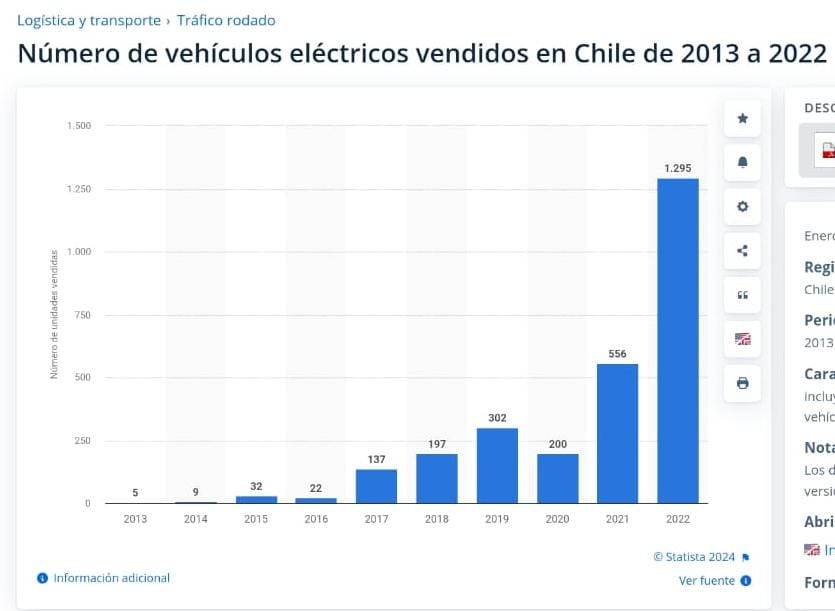
\includegraphics[scale=0.4]{imagenes/grafica-1}
		\caption{Número de vehículos eléctricos vendidos en Chile entre 2013 y 2022. \cite{statista}}
		\label{fig:grafica1}
	\end{figure}

	\begin{figure}[htbp]
		\centering
		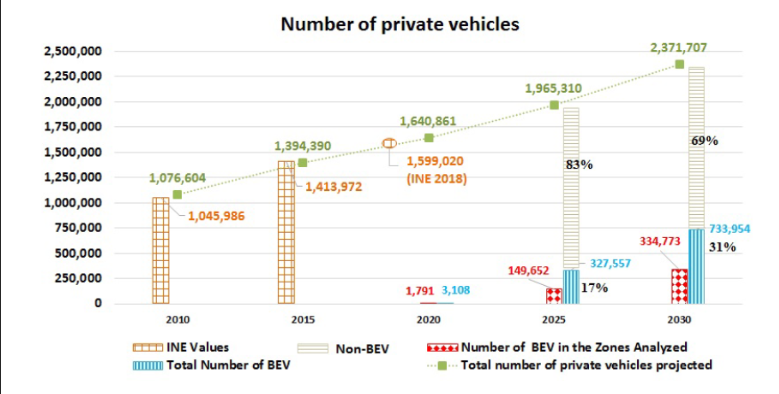
\includegraphics[scale=0.5]{imagenes/grafica-2}
		\caption{Número de autos privados \cite{paredes}}
		\label{fig:grafica2}
	\end{figure}
	\newpage
	\begin{figure}[htbp]
		\centering
		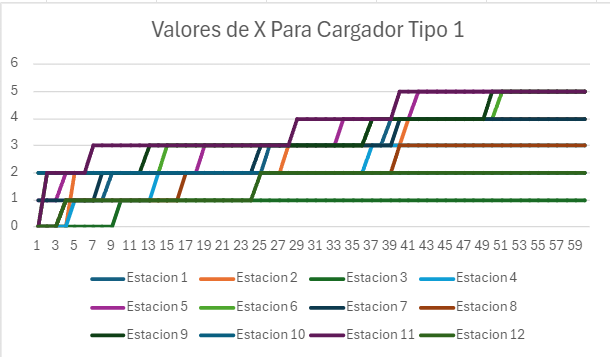
\includegraphics[scale=0.9]{imagenes/anexo_xmit1.png}
		\caption{Gráfico 1 de la variable $x_{mit}$.}
		\label{fig:grafica3}
	\end{figure}

	\begin{figure}[htbp]
		\centering
		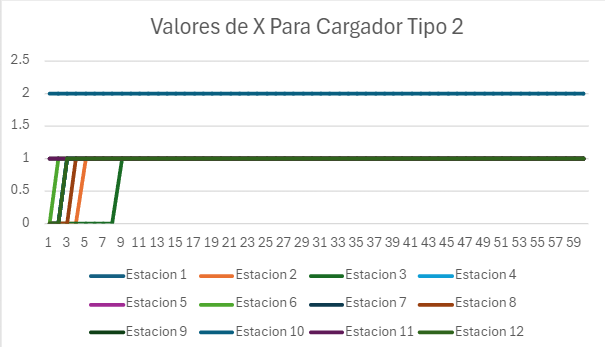
\includegraphics[scale=0.9]{imagenes/anexo_xmit2.png}
		\caption{Gráfico 2 de la variable $x_{mit}$.}
		\label{fig:grafica4}
	\end{figure}
	\newpage

	\begin{figure}[htbp]
		\centering
		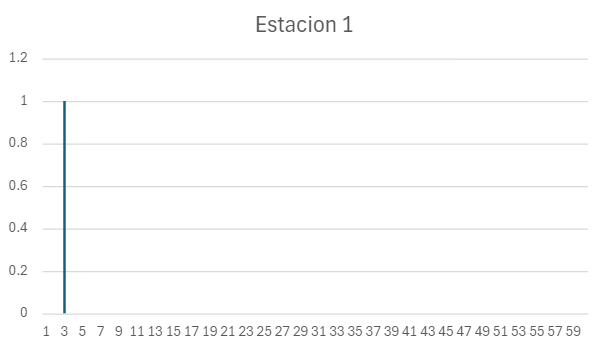
\includegraphics[scale=0.9]{imagenes/ymit1.png}
		\caption{Gráfico 1 de la variable $y_{mit}$.}
		\label{fig:grafica5}
	\end{figure}
	\begin{figure}[htbp]
		\centering
		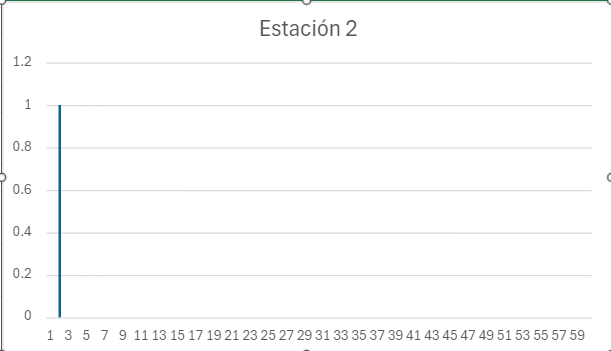
\includegraphics[scale=0.9]{imagenes/ymit2.png}
		\caption{Gráfico 2 de la variable $y_{mit}$.}
		\label{fig:grafica6}
	\end{figure}
	\newpage

	\begin{figure}[htbp]
		\centering
		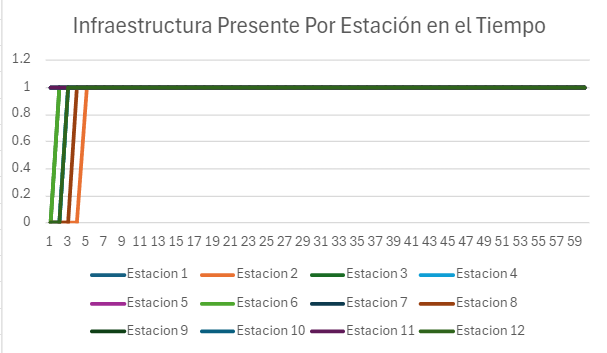
\includegraphics[scale=0.9]{imagenes/zit.png}
		\caption{Gráfico de la variable $z_{it}$.}
		\label{fig:grafica7}
	\end{figure}

	\begin{figure}[htbp]
		\centering
		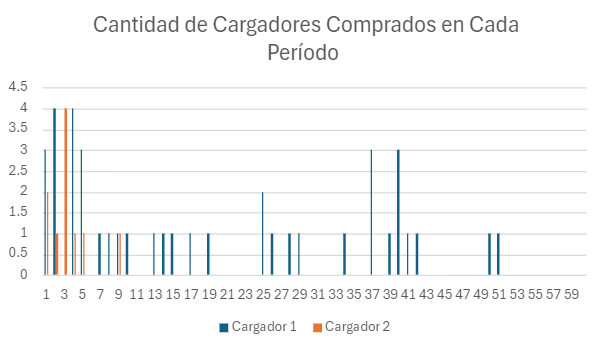
\includegraphics[scale=0.9]{imagenes/amt.png}
		\caption{Gráfico de la variable $a_{mt}$.}
		\label{fig:grafica8}
	\end{figure}
	\newpage

	\begin{figure}[htbp]
		\centering
		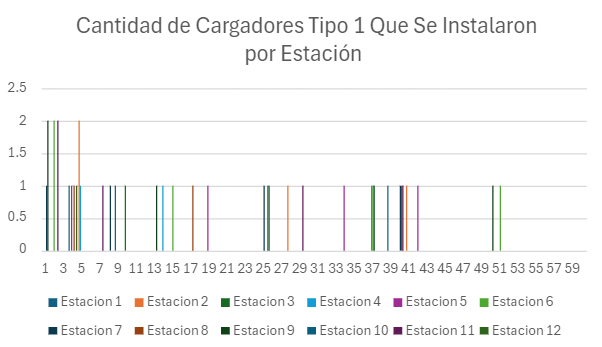
\includegraphics[scale=0.9]{imagenes/bmit1.png}
		\caption{Gráfico 1 de la variable $b_{mit}$.}
		\label{fig:grafica9}
	\end{figure}

	\begin{figure}[htbp]
		\centering
		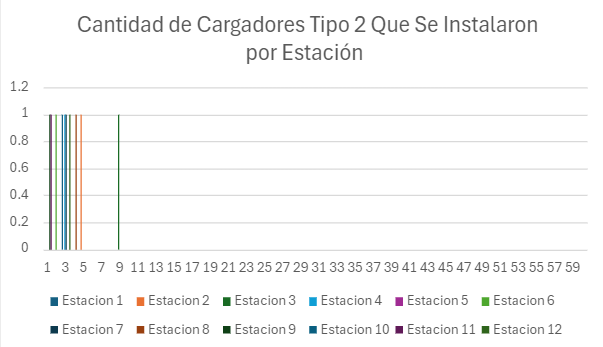
\includegraphics[scale=0.9]{imagenes/bmit2.png}
		\caption{Gráfico 2 de la variable $b_{mit}$.}
		\label{fig:grafica10}
	\end{figure}
	\newpage


	\begin{figure}[htbp]
		\centering
		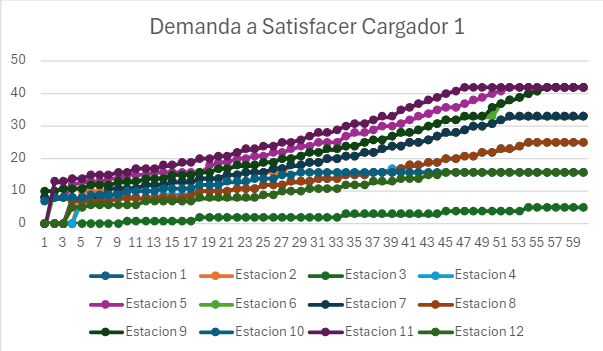
\includegraphics[scale=0.6]{imagenes/dmit1.png}
		\caption{Gráfico 1 de la variable $d_{mit}$.}
		\label{fig:grafica11}
	\end{figure}

	\begin{figure}[htbp]
		\centering
		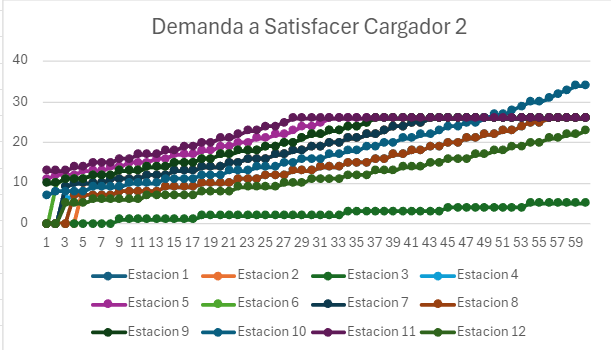
\includegraphics[scale=0.6]{imagenes/dmit2.png}
		\caption{Gráfico 2 de la variable $d_{mit}$.}
		\label{fig:grafica12}
	\end{figure}

	\begin{figure}[htbp]
		\centering
		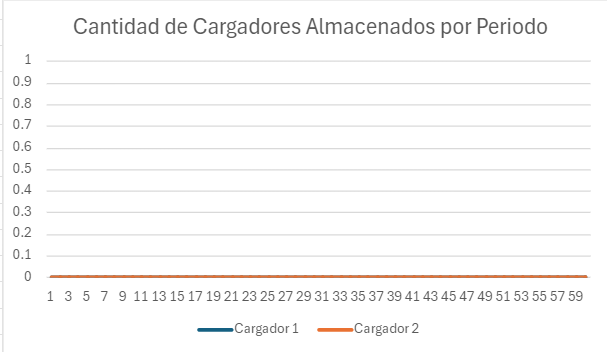
\includegraphics[scale=0.6]{imagenes/smt.png}
		\caption{Gráfico de la variable $S_{mt}$.}
		\label{fig:grafica13}
	\end{figure}

\end{flushleft}
\end{document}
